\documentclass[spanish,english,12pt,letterpaper,oneside]{book}
\usepackage{layout}
\usepackage[spanish]{babel}
\usepackage{calc}
\usepackage[latin1]{inputenc}
\usepackage{latexsym}
\usepackage{amssymb}
\usepackage{fancybox}
\usepackage{fancyvrb}
\usepackage{fancyhdr}
\usepackage{relsize}
\usepackage{pgf,pgfarrows,pgfnodes}
\usepackage{tikz}
\usepackage{rotating}
\usepackage{tabularx}
\usepackage{color}
\usepackage{float}
\usepackage{index}
%\usepackage{wasysym}
\usepackage{amsmath}
\usepackage{multirow}
\usepackage{listings}
\usepackage[pdftex,hyperindex,breaklinks]{hyperref}%,colorlinks,urlcolor=blue,linkcolor=blue]{hyperref}

\usepackage[left=4cm,top=3.0cm,right=3.4cm,bottom=3.9cm]{geometry}

%Para activar el doble espacio
%\renewcommand{\baselinestretch}{2} 

\usepackage[ruled,Algoritmo]{algorithm}

%\usepackage[noend]{algpseudocode}
\usepackage{algpseudocode}







\usepackage{algpseudocode}
%%%%%%%%%%%%%%%%%%%%%%%%%%%%%%%%%%%%%%%%%%%%%%%%%%%%%%%%%%
% NEW PACKAGES INTRODUCED BY LSC FOR REVIEWING PURPOSES
%\usepackage{ulem}
%\usepackage{boxedminipage}
%%%%%%%%%%%%%%%%%%%%%%%%%%%%%%%%%%%%%%%%%%%%%%%%%%%%%%%%%%%

%----------MY_\em-STYLE theorems -------------
%%% http://www.stat.umn.edu/~charlie/amslatex.html#theorem
%\usepackage{amsthm}
%\newtheoremstyle{itarikaj}
%{2ex}%   Before skip
%{2ex}%   After skip
%{\footnotesize\sl }%      Body font (empty=\rm)
%{}%      Indent amount (empty=no indent, \parindent=para indent)
%{\footnotesize\bf\itshape}%   Thm head font
%{:}%     Punctuation after thm head
%{1em}%   Space after thm head (\newline=linebreak)
%{}%      Thm head spec (can be left empty, meaning `normal')
%{ }%\thmname{#1}\thmnumber{ #2}\thmnote{ #3} }% Thm head spec
%\theoremstyle{itarikaj}
%\newtheorem{nudecom}{Comentario-LS-}
%\newtheorem{myrem}{Remark}

%%%%%%%%%%%%%%%%%%%%%%%%%%%%%%%%%%%%%%%%%%%%%%%%%%%%%%%%%%
% NEW ENVIRONMENT INTRODUCED BY LSC FOR REVIEWING PURPOSES
%\newenvironment{com}%
%{\mbox{} \\
 % \begin{flushleft}\begin{boxedminipage}[t]{120mm}\begin{nudecom}}
%{\end{nudecom}\end{boxedminipage}\end{flushleft}}
%%%%%%%%%%%%%%%%%%%%%%%%%%%%%%%%%%%%%%%%%%%%%%%%%%%%%%%%%%








\renewcommand{\headrulewidth}{1pt}
%\renewcommand{\footrulewidth}{0.5pt}


\newcounter{myfootertablecounter}

\newcommand\myfootnotemark{%
  %\refstepcounter{footnote}%
  \addtocounter{footnote}{1}%
  \footnotemark[\thefootnote]%
}%

\newcommand\myfootnotetext[1]{%
  \addtocounter{myfootertablecounter}{1}
  \footnotetext[\value{myfootertablecounter}]{#1}
}

% from now on, myfootnote has to be used rather than footnote to
% adapt the myfootercounter
\newcommand\myfootnote[1]{%
  \addtocounter{myfootertablecounter}{1}
  \footnote{#1}
}%


\pagestyle{fancy}

\rhead[]{\leftmark}
\lhead[\rightmark]{}
%\lfoot[\thepage]{ATLAS Grid Information System}
\rfoot[ATLAS Grid Information System]{\thepage}
\cfoot{} 


%\renewcommand{\listalgorithmname}{\'Indice de algoritmos}
\renewcommand{\chaptermark}[1]{\markleft{\thechapter #1}}
\renewcommand{\sectionmark}[1]{\markright{\thesection #1}}
\renewcommand{\chaptermark}[1]{\markboth{\chaptername \ \thechapter. #1}{}}

\newcommand{\contrib}[3]{#1\quad$<$\texttt{#2}$>$%
{\small\\\quad\textit{#3}}\\[1ex]}

\pgfdeclareimage[width=3cm]{logo-utfsm}{images/logo-utfsm}
\pgfdeclareimage[width=11cm]{trigger}{images/trigger2}
\pgfdeclareimage[width=11cm]{tiercloud}{images/tiercloud3}
\pgfdeclareimage[width=5cm]{atlasoverview}{images/atlasoverview2}

\pgfdeclareimage[width=7cm]{gridArchitecture}{images/gridArchitecture2}
\pgfdeclareimage[width=12cm]{GT4figure}{images/GT4figure}
\pgfdeclareimage[width=10cm]{gLitefigure}{images/gLitefigure2}
\pgfdeclareimage[width=12cm]{ARCarch}{images/Arc-architecture}

\pgfdeclareimage[width=10cm]{apel}{images/apel}
\pgfdeclareimage[width=10cm]{sgas}{images/sgas}
\pgfdeclareimage[width=6cm]{accsys}{images/accsys}
\pgfdeclareimage[width=8cm]{apelCollector}{images/apelCollector2}
\pgfdeclareimage[width=8cm]{gratiaCollector}{images/gratiaCollector2}
\pgfdeclareimage[width=10cm]{databaseSchemaAPEL}{images/databaseSchemaAPEL}

\pgfdeclareimage[width=7cm]{MDS2}{images/MDS2v2}
\pgfdeclareimage[width=10cm]{GRISGIIS}{images/GRISGIIS}
\pgfdeclareimage[width=7cm]{BDII}{images/BDII2}
\pgfdeclareimage[width=5cm]{BDIIInstance}{images/bdiiTWiki}
\pgfdeclareimage[width=14cm]{ARCTree}{images/ARCTree}
\pgfdeclareimage[width=8cm]{RGMA}{images/R-GMA}
\pgfdeclareimage[width=12cm]{RGMAVirtual}{images/virtual_db}
\pgfdeclareimage[width=10cm]{MDS4DataFlow}{images/webServiceGIS}



\pgfdeclareimage[width=8cm]{DDMarchitecture}{images/ddmArchitecture}
\pgfdeclareimage[width=8cm]{pandaOverview}{images/pandaoverview}
\pgfdeclareimage[width=8cm]{ToACVS}{images/ToACVS}
\pgfdeclareimage[width=11cm]{AGISArchitecture}{images/AGISArchitecture5}
%\pgfdeclareimage[width=11cm]{databaseSchemaAGIS}{images/EntityRelationship}
\pgfdeclareimage[width=11cm]{databaseSchemaAGIS}{images/databaseSchemaAGIS}

\pgfdeclareimage[width=10cm]{plotGetCloud50}{images/cloudTest10SMCU50}
\pgfdeclareimage[width=12cm]{plotGetCloud25}{images/cloudTest10SMCU25}
\pgfdeclareimage[width=12cm]{plotGetCloud75}{images/cloudTest10SMCU75}
\pgfdeclareimage[width=12cm]{plotGetCloud100}{images/cloudTest10SMCU100}
\pgfdeclareimage[width=16cm]{plotSite25}{images/siteTest10SMCU25}
\pgfdeclareimage[width=16cm]{plotSite50}{images/siteTest10SMCU50}
\pgfdeclareimage[width=16cm]{plotTopo25}{images/topologyTest10SMCU25}
\pgfdeclareimage[width=16cm]{plotTopo50}{images/topologyTest10SMCU50}

\pgfdeclareimage[width=10cm]{plotService}{images/plotService}
\pgfdeclareimage[width=10cm]{plotTopology}{images/plotTopology}


\pgfdeclareimage[width=14cm]{RDFAGISArchitecture}{images/RDFAGISArchitecture}
\pgfdeclareimage[width=10cm]{RDPComponent}{images/RDPComponent}
\pgfdeclareimage[width=8cm]{RDFgraph}{RDFgraph}
\pgfdeclareimage[width=14cm]{coregrid}{images/coregrid}
\pgfdeclareimage[width=14cm]{ATLASontology}{images/ATLASontology}
\pgfdeclareimage[width=7cm]{hybrid}{images/hybrid}


%\addto\captionsspanish{%
%  \def\listtablename{\'Indice de tablas}%
%  \def\tablename{Tabla}%
%}


\title{3D Scene Reconstruction}

\author{
  Juan Reyes \\ \texttt{jareyes@alumnos.inf.utfsm.cl}
}

\date{$\infty$}

\frenchspacing

\makeindex

\begin{document}
\frontmatter

\thispagestyle{empty}

\begin{center}

{\large\bfseries Universidad T�cnica Federico Santa Mar�a}\\[2mm]
{\large\bfseries Departamento de Inform�tica}\\[2mm]
\pgfuseimage{logo-utfsm}
\end{center}

\vspace*{\stretch{3}}

\begin{center}
{\LARGE\bfseries 3D Scene Reconstruction }\\[2mm]
%{\LARGE\bfseries Using a Kinect sensor}
\end{center}

\vspace*{\stretch{5}}

\begin{center}
{\large por}\\[2mm]
{\huge Juan Alfonso Reyes L�pez}
\end{center}


\vspace*{\stretch{5}}

\begin{center}
{\large Tesis para optar al  grado de}\\[2mm]
\vspace*{10mm}
{\LARGE Mag�ster en Ciencias de la Ingenier�a Inform�tica}\\[2mm]
%{\large for the degree of}\\
%{\Large Master in Science of Informatic Engineering}
\end{center}

\vspace*{\stretch{5}}


\begin{center}
{\large Valpara\'{i}so - Chile}\\
{\large Marzo de 2015}\\[2mm]
\end{center}

\vspace*{\stretch{1}}

\pagebreak

\thispagestyle{empty}

\begin{center}
{\Large Universidad T\'{e}cnica Federico Santa Mar\'{\i}a} \\
{\Large Departamento de Inform�tica}\\
{\Large Valpara\'{\i}so - Chile}\\
\end{center}

\vspace*{\stretch{1}}

\begin{center}
{\large TITULO DE LA TESIS:}\\
{\large \textbf{3D Scene Reconstruction}}
\end{center}

\vspace*{\stretch{1}}

\begin{center}
{\large AUTOR:}\\
{\large \textbf{Juan Alfonso Reyes L�pez}}\\
\end{center}

\vspace*{\stretch{2}}

{\large TRABAJO DE GRADO, presentado en cumplimiento parcial de los
requisitos para el Grado de
Mag�ster en Ciencias de la  Ingenier�a Inform�tica de la Universidad T�cnica Federico
Santa Mar�a.}

\vspace*{\stretch{5}}

\begin{table}[ptbh]
\begin{tabular}[c]{lc}
{\large Prof. Dr. Luis Salinas} & \begin{picture}(200,5) \line(1,0){200} \end{picture}\\
& {\large Profesor Gu�a } \\
& \\
& \\
& \\
{\large Prof. Dr. Claudio Torres } & \begin{picture}(200,5) \line(1,0){200} \end{picture} \\ 
& {\large Correferente } \\
& \\
& \\
& \\
{\large Dr.} & \begin{picture}(200,5) \line(1,0){200} \end{picture}\\
& {\large Correferente Externo }
\end{tabular}
\end{table}

\vspace*{\stretch{1}}

\begin{center}
{\large Marzo de 2015}
\end{center}
 
\pagebreak


\endinput


\chapter*{Abstract}

3D point cloud registration is an important step in every 3D reconstruction system. This thesis proposes to register 
3D point clouds, applying a filtering step where only edges that appear 
in the two point clouds to be aligned pass the filter. For this purpose a combination of visual and geometrical information is 
used along with the Iterative Closest Point (ICP)
  algorithm and a pose graph optimization method. The proposed technique reduces the amount of calculations 
involved because only between 10\% and 20\% of original points are used as input for the ICP algorithm, increasing 
the quality of the alignment, working with the most representative subset of the data. At difference to other techniques 
involving edge filtering along with ICP, this proposal increments the odds of a correct alignment filtering out non common 
data from the pair of point clouds to be aligned. Quantitative results shows the advantages of the proposed method. A 
public available dataset was used, 
providing the source 
code and all the necessary information to compare and replicate the presented results.

\section*{Keywords}

3D reconstruction, simultaneous location and mapping, iterative closest point, Kinect, point cloud


\addcontentsline{toc}{section}{\contentsname}
\tableofcontents

%\addcontentsline{toc}{subsection}{\listalgorithmname}
%\listofalgorithms
\addcontentsline{toc}{subsection}{\listfigurename}
\listoffigures
\addcontentsline{toc}{subsection}{\listtablename}
\listoftables

\mainmatter

\chapter{Introducction}
\label{introduccion}
\index{Introducction}

The 3D scene reconstruction problem consists in take the
necessary information from a real scene in order to reconstruct
it in a three dimensional space, usually to be displayed 
in a computer. 

The objetive is to represent in the most accurate way the geometric scene details, obtaining rich 
information about the scene that is not explicity contained on a single image and then use this 
to reconstruct the scene or use it to perform a more advanced task that depends of the scene geometry. 
Some applications of 3D scene reconstruction are : Autonumous vehicle or robot navigation, where there is crucial to have 
the scene geometry in order to locate paths and obstacles. Augmented Reallity, where a virtual 3D object
 is added to a real video of the scene. Parts inspection in a manufacturing plant, where is necesary to detect
 fabrication defects on some objects. Statues and Buildings preservation, in order to have a digital representation 
of the objects and beign able to reproduce or mantain them.

 
In general the information is acquired
 from the scene with optical devices, such as RGB cameras or depth sensors.
Most of 3D scene reconstruction methods can be classified in passive methods and active methods \cite{lanman}.
The passive methods works without controlling the light in the scene, they just receipt light (ordinary cameras). 
By the other hand active methods alter the light in the scene, with a light emisor and its corresponding 
receptor, projecting patterns of light in order to simplify the matching process prior to the triangulation. 
There are also some active methods that touch the object in order to reconstruct it, but they are beyond 
the scope of this thesis. 

The most accurate and expensive method to perform 3D scene reconstruction is the Laser Scanning, because it has 
an hight accuracy (about xx mm). But nowadays there are emerging cheaper devices that potentially could perform 
a similar reconstruction at a pair of orders of magnitude low cost. 

One of the most classical approaches is to use multiple 2D
 images taken from known camera viewpoints and estimate the distance of each
 relevant pixel with triangulation (Stereo Vision, Multiview Vision), with this 
approaches the depth map must be generated using the geometrical information contained
 on the images. Nowadays is common to find devices that generate depth maps accesible
 to everyday users and automatize the depth map generation step, this devices are called depth sensors. 
Depth sensors give to each pixel of the image a depth value, related
with the distance of the real object from the sensor, offering a more
accurate data to perform 3D reconstruction. With the appearance
of cheap depth sensors for gaming and entertainment (such as
Kinect). There is a growing interest in the develop of low cost
3D reconstruction systems. 


One of the key steps of a 3D reconstruction algorithm is the registration, where the 3D points corresponding to
 the scene are  registered in a common coordinate system, preserving the original scene disposition. Another important 
step is to add colour and continuity to the reconstructed scene, usually using a lot of geometric primitives such as 
triangles, in order to generate a textured 3D model. This thesis is  about the registration step. 




\chapter{State of Art}
\index{State Of Art}
 
Nowadays there is a growing interest on the 3D scene reconstruction field, due to the incresing computational power and the reduction of 
the costs of the capturing devices. There are a lot of differents approaches to afront the problem, there are works that perform 3D reconstruction 
from a video, from a set of images taken with an unknown camera and orientation, using active devices that project patterns of light into 
the scene, lasers, etc. 

In 3D reconstruction an important part of the problem depends of the intrinsical 
device characteristics (noise, resolution, framerate, etc), the scene or object beign captured, ilumination, the camera location and position, etc. All this factors configure different instances of the problem, difficulting the comparison and limiting the use of a common dataset, but some efforts in order to allow comparison between different algorithms has been made 
in \cite{seitz2006}, \cite{ponce2006} and \cite{scharstein2001}.

Usually the researchers estimate their systems performance comparing the generated 3D model with some 
ground truth model obtained with a high precision laser scanner. Also its common to measure the performance
 comparing some result obtained at an intermediate step of the reconstruction process with a ground truth measure, 
such as the camera estimated path with camera real path.   

%done
Reconstruction from a set of photographs without human assistance is performed in \cite{jan}, they demonstrated the first system able to deliver dense geometry for Internet scale photo collections with millions of images of an entire city within the span of a day on a single PC. They used appearance-based clustering in multiple CPU and GPU cores 
in order agrupate images corresponding to the same site, using gist features for each image along with a RGB
descriptor in order to mantain color information. They also used geo-location information available for some of 
the images. Then at each cluster they performed 3D reconstruction using only the images with mutually consistent epipolar 
geometry. From millions of images from one city they generated thousands of 3D models of buildings. See figure \ref{fig:jan}. 


\begin{figure}[h!]
\begin{center}
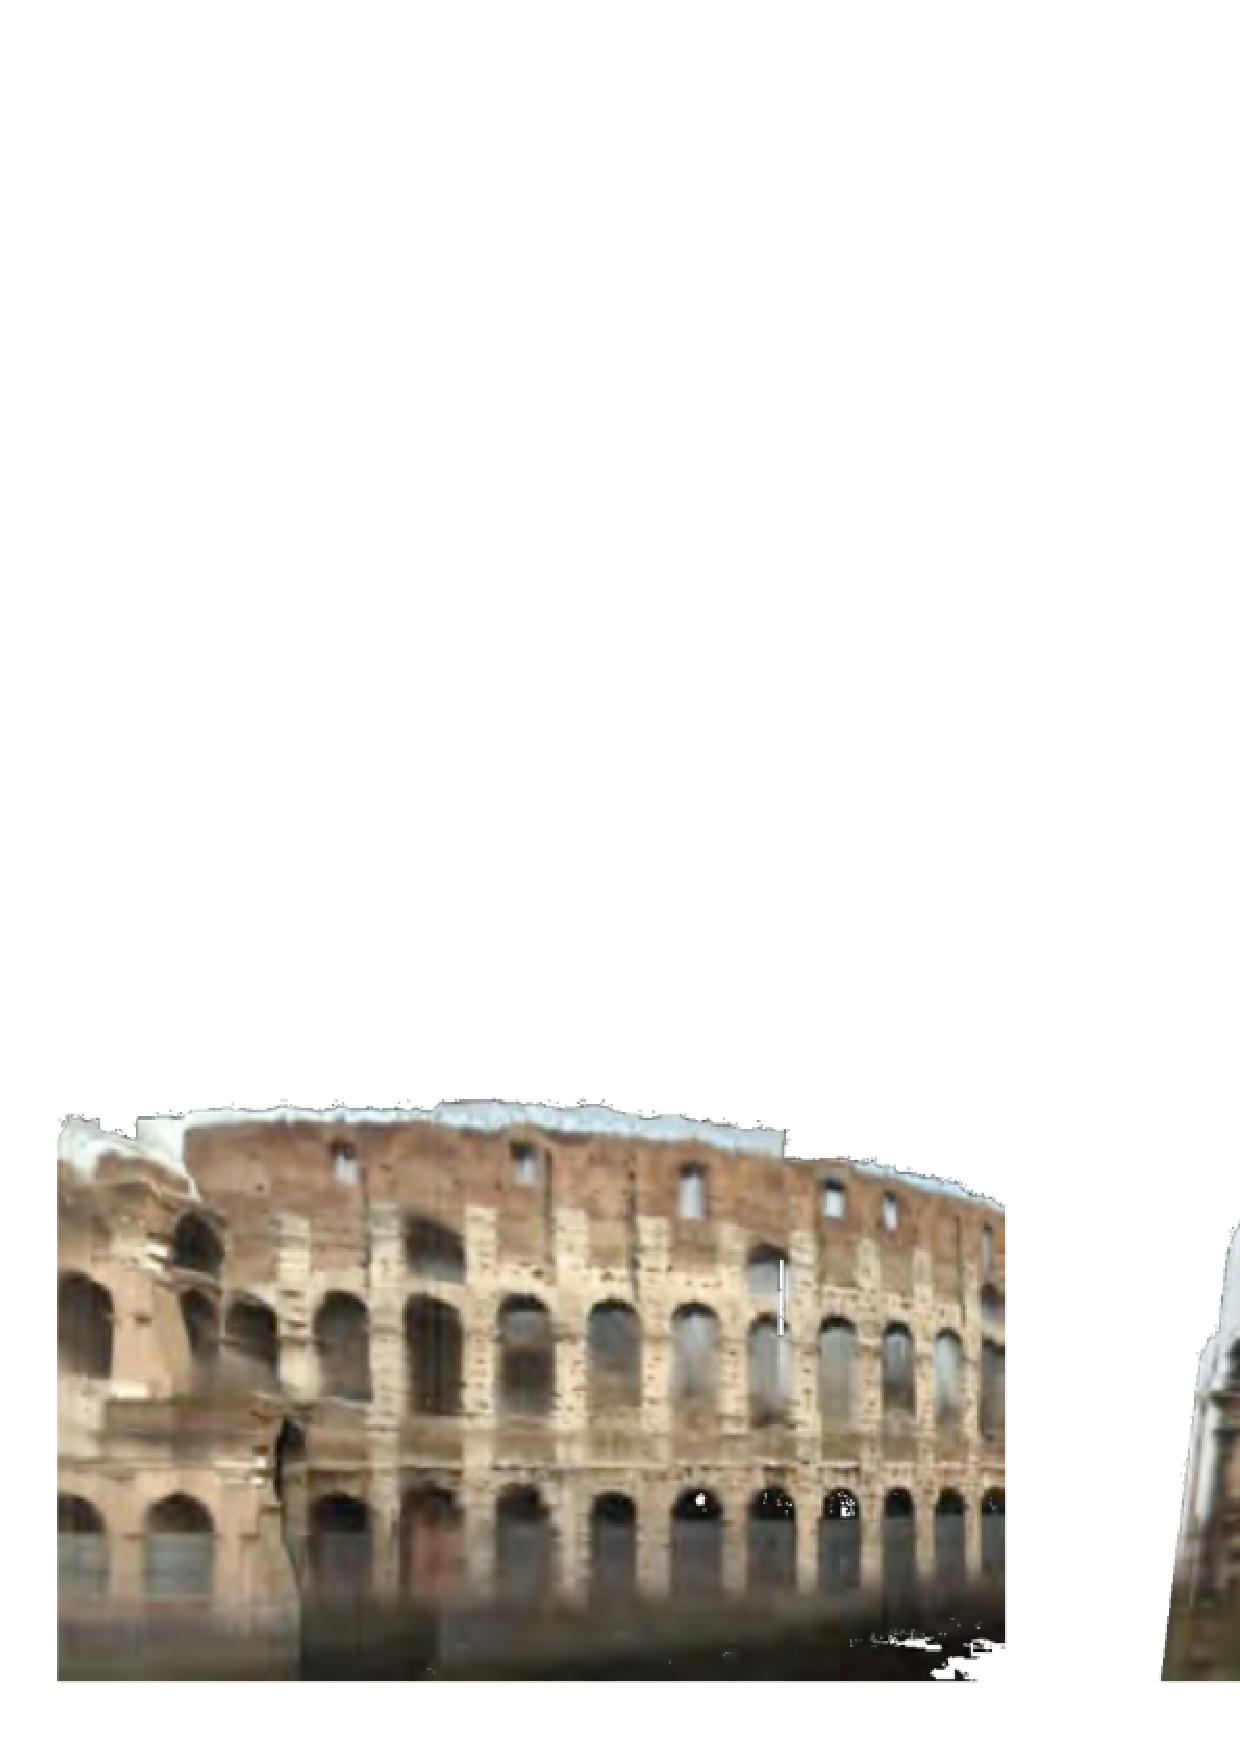
\includegraphics[scale=0.25]{images/jan}
\caption{Reconstructed 3D buildings in less than 24 hr. using 2.8 million and 2.9 million of images respectively}
\label{fig:jan}
\end{center}
\end{figure}

%done
In \cite{guangyu} an hybrid approach is used, combining a ToF (Time of Flight) camera and an grayscale camera in order to perform the reconstruction. 
The data adquisition is made rotating the object in front of the camera with a black background behind it, then they use 
SIFT (Scale Invariant Feature Transform) to find 2D feature correspondences and perform and initial alination between two consecutive frames, this alineation is 
then improved with ICP (Iterative Closest Point) algorithm. They use a 3D laser scanner in order to obtain a ground truth, obtaining a difference around of 1\% 
between their reconstructed
 models and the 3D laser models. See figure \ref{fig:guangyu}.

%put this on the correct place
Its common to find works where the method is not quantitatively evaluated 
in 3D reconstruction due to the high 
cost of a laser scanner that is used as ground truth. 


\begin{figure}[h!]
\begin{center}
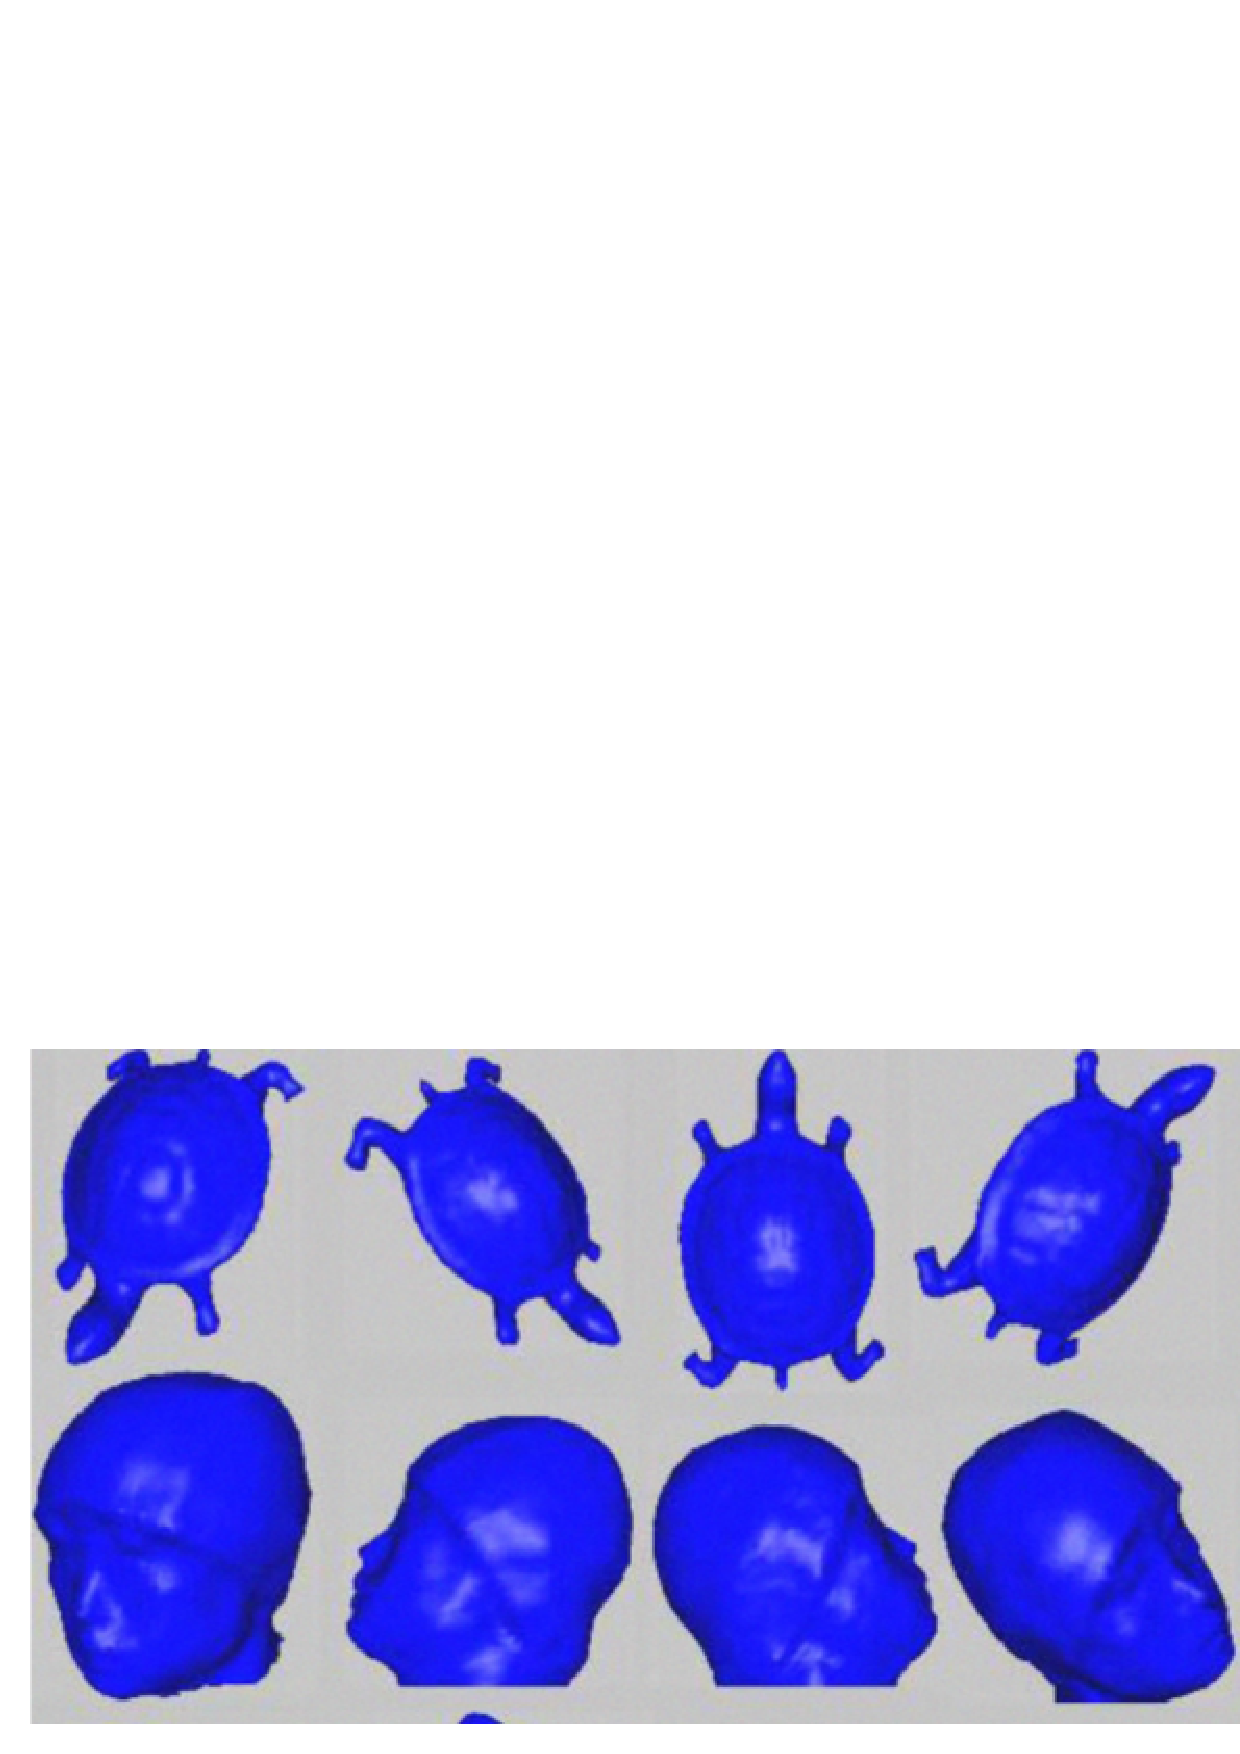
\includegraphics[scale=0.38]{images/guangyu}
\caption{3D Reconstruction of a human head and an object using ToF and RGB camera}
\label{fig:guangyu}
\end{center}
\end{figure}

%done
In \cite{may2009} a ToF camera is used in combination with an industrial robot arm (KUKA KR 16) in order to register an indor scene,
they use an improved version of the ICP algorithm called ICP Frustum, where at each iteration the points that are not overlaping with the previous frame are removed. The industrial robot arm is used to move the camera and get a ground truth camera path to evaluate the performance of their ICP algorithm. 

%Its possible to find more elaborated reconstructions using a laser scanner, but its a more expensive method. In 
%\cite{binney} there is a interesting work where a reconstruction of tree branches is performed using a laser range 
%data. They use a probabilistic approach and use knowledge about the tree structure to guide an iterative reconstruction 
%process. 

%done
In \cite{keqiang} a 3D reconstruction is performed with a laser range finder (SICK 2D ) and a mobile robot, 
using the ICP algorithm and a volumetric representation. In the matching phase of the ICP algorithm not all
 points are used, instead they just use edge points, reducing the computational cost of the process. The scene 
 representation is simplyfied removing redundant points, this is done dividing the scene into voxels and at each 
 voxel preserving just the point closer to the center. Their system produces a scene with data points evenly 
 distributed.

%revisar nuevamente
In \cite{wei} a CCD camera and a 2D laser scanner is used to perform indoor panoramic 3D reconstruction, 
they mounted both devices in a rotational stage and use a fusion algorithm to merge the depth map generated by the laser 
and the depth map generated from the CCD camera observations, the two depth maps contains noise and an intelligent merging reduce this
 noise giving more accurate information to the 3D reconstruction process. Another interesting work of indoor scene reconstruction is \cite{henry} where an RGB-D camera is used to reconstruct an indoor scene. RGB-D cameras are sensing systems that capture RGB images
 along with per pixel depth information. They use the ICP algorithm to calculate the camera location and pass to it information from 
the depth camera and  rich visual
 features along with RANSAC (RAndom SAmple Consensus) verification captured by the RGB camera. They use surfels \cite{pfister} to represent the scene. See figure \ref{fig:henry}.

\begin{figure}[h!]
\begin{center}
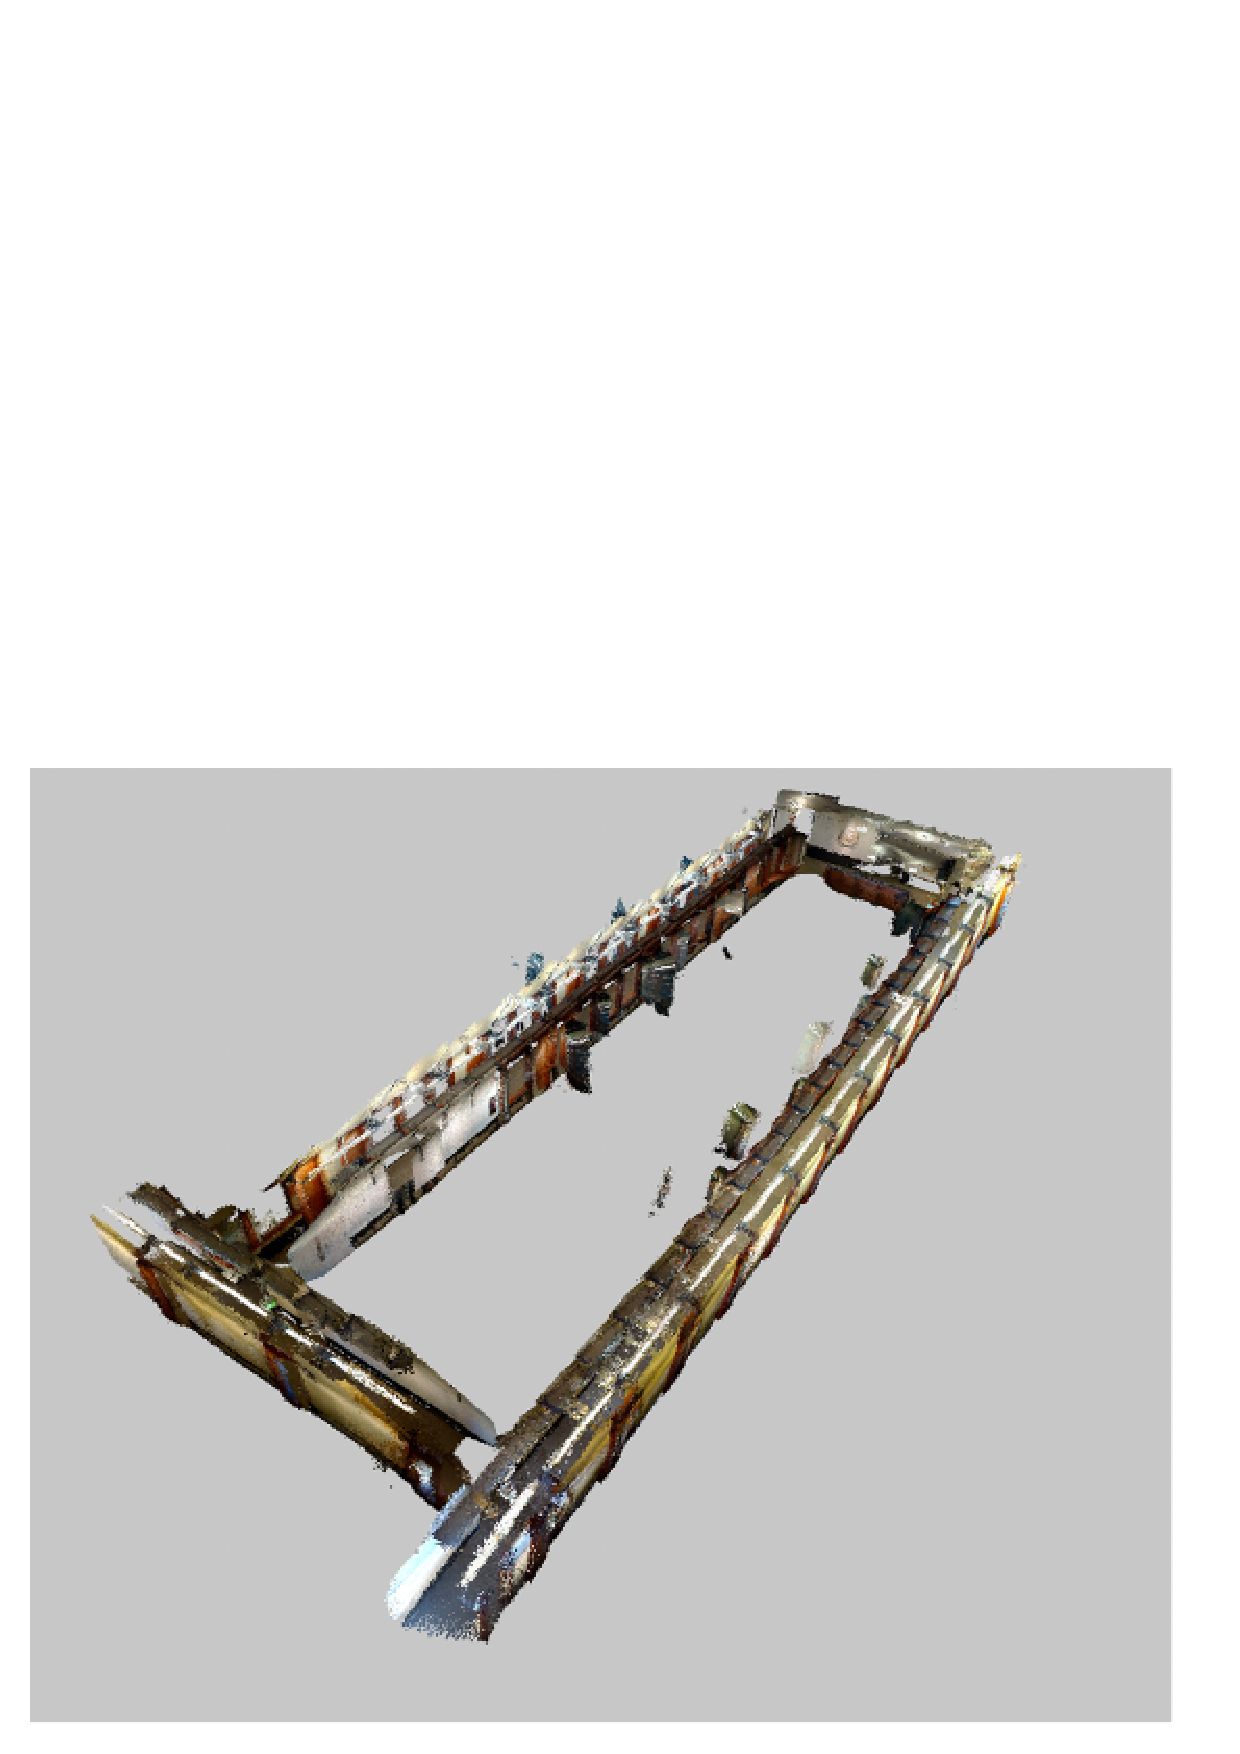
\includegraphics[scale=0.29]{images/henry}
\caption{Reconstructed 3D big indoor space}
\label{fig:henry}
\end{center}
\end{figure}

%done
In \cite{cui} a ToF camera is used to reconstruct 3D objects. A combination of 3D superresolution method with a 
probabilistic scan alignment (iterative Expectation Maximization) approach that takes into account the sensor's 
noise characteristics is used. Their method is not in real time and the resulting models contains undesirable 
artifacts due to  the noise of the captured depth maps, they use a low resolution device (176x144) and they 
improve the resolution using a superresolution method. They captured a ground truth model with a laser 3D scanner, 
obtaining differences below 1 cm in most areas between their model and the ground truth model. Their scanning 
procedure doesn't allow a freely movement around the object, the object must be at the center of view of the camera 
and the distance between the object and camera must be almost constant. A similar work can be found at \cite{schoun} where 
 a hierarchical Lukas Kanade optical flow is used for registration.
 
see figure \ref{fig:cui}.

\begin{figure}[h!]
\begin{center}
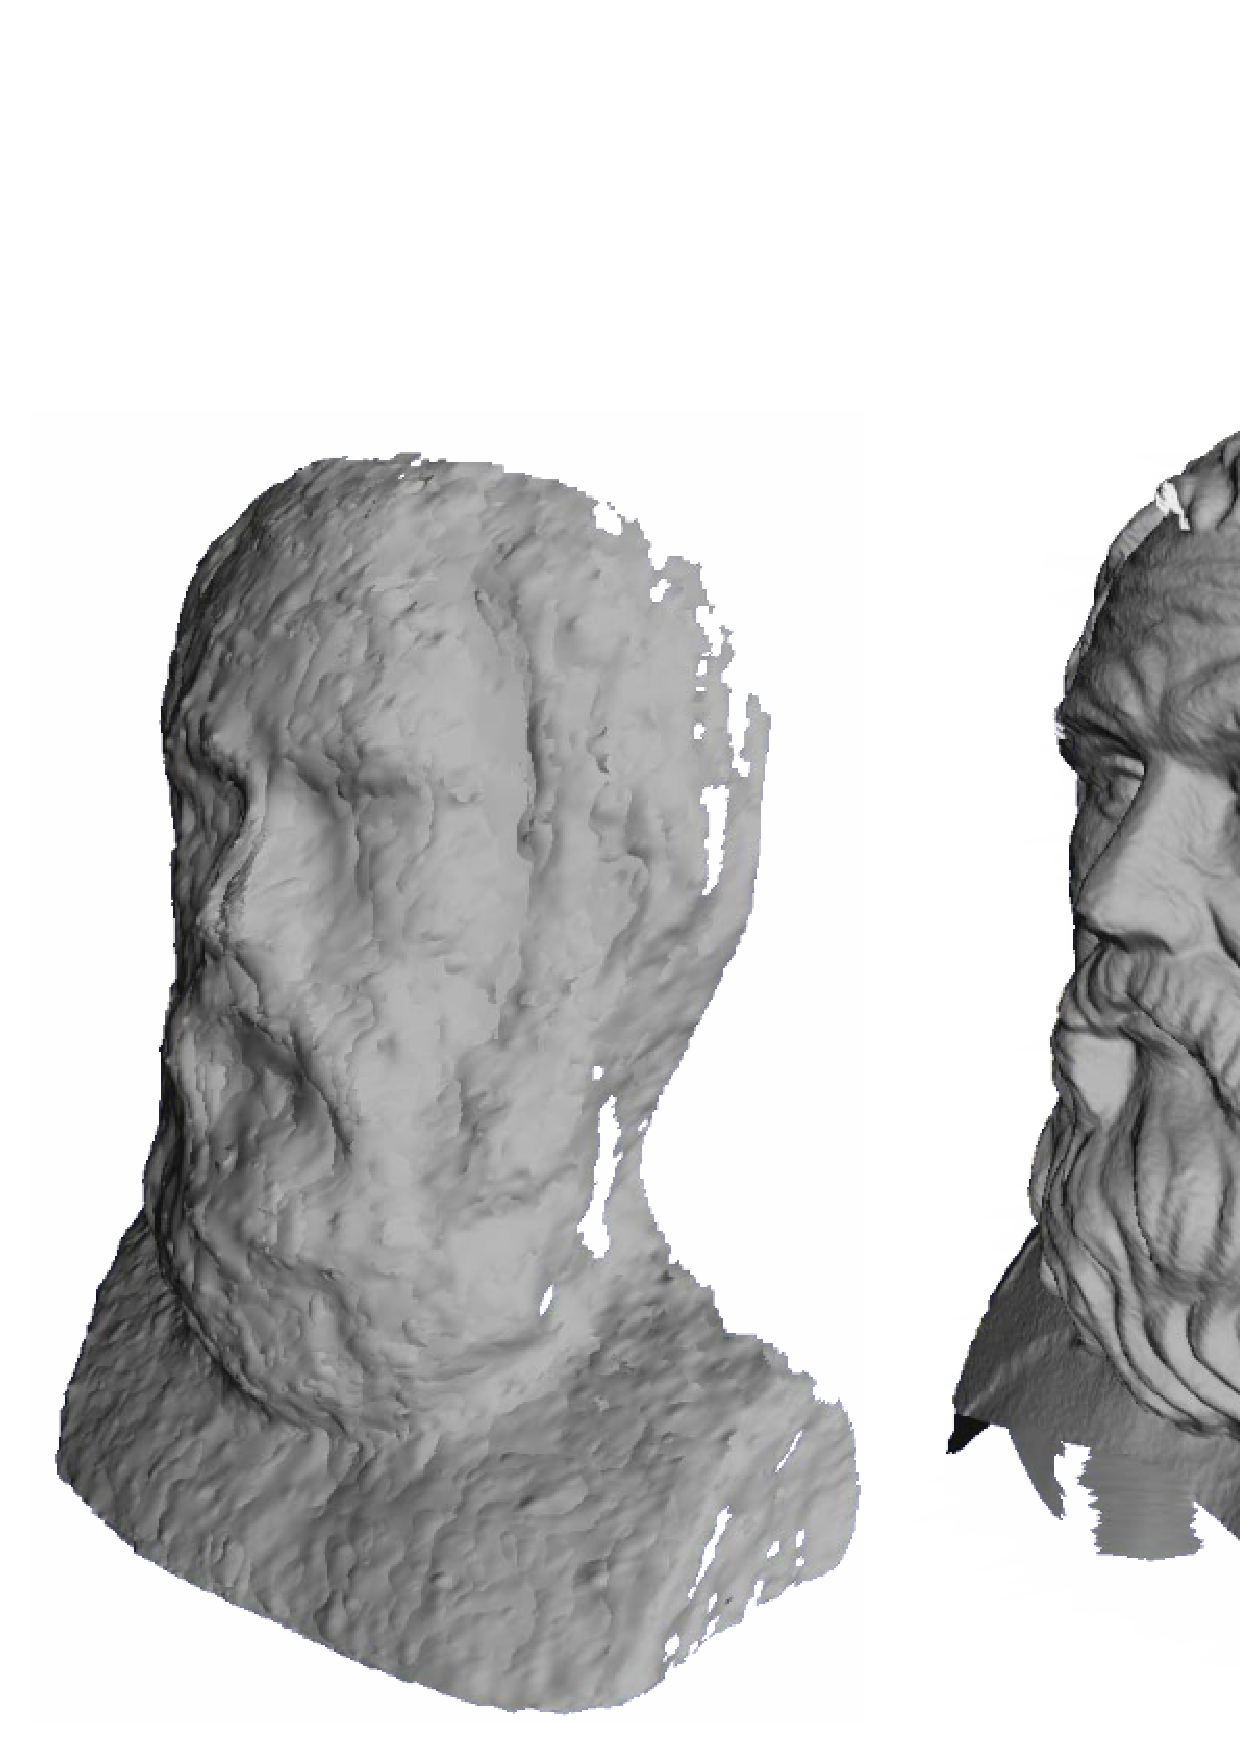
\includegraphics[scale=0.23]{images/cui}
\caption{ToF Reconstruction, Laser Reconstruction and Error Plot}
\label{fig:cui}
\end{center}
\end{figure}

 
%done
A very interesting work is made in \cite{izadi}, they use a low cost RGB-D camera (Kinect) in order to perform
the 3D reconstruction using the ICP algorithm  and a volumetric representation with a GPU in order to 
archieve real time reconstruction. The camera can move freely around the scene and the reconstruction grows in detail 
as new depth measurements are added. They apply color textures to the reconstructed scene obtaining very 
realistic models, their system is able to perform rigid body collisions 
simulations during the reconstruction, allowing thousands of virtual particles interact with the scene. Also a 
user can interact with the scene during the reconstruction process. This is one of the most advanced 
reconstruction systems, due to its uniques features.

 see figure \ref{fig:izadi}.

\begin{figure}[h!]
\begin{center}
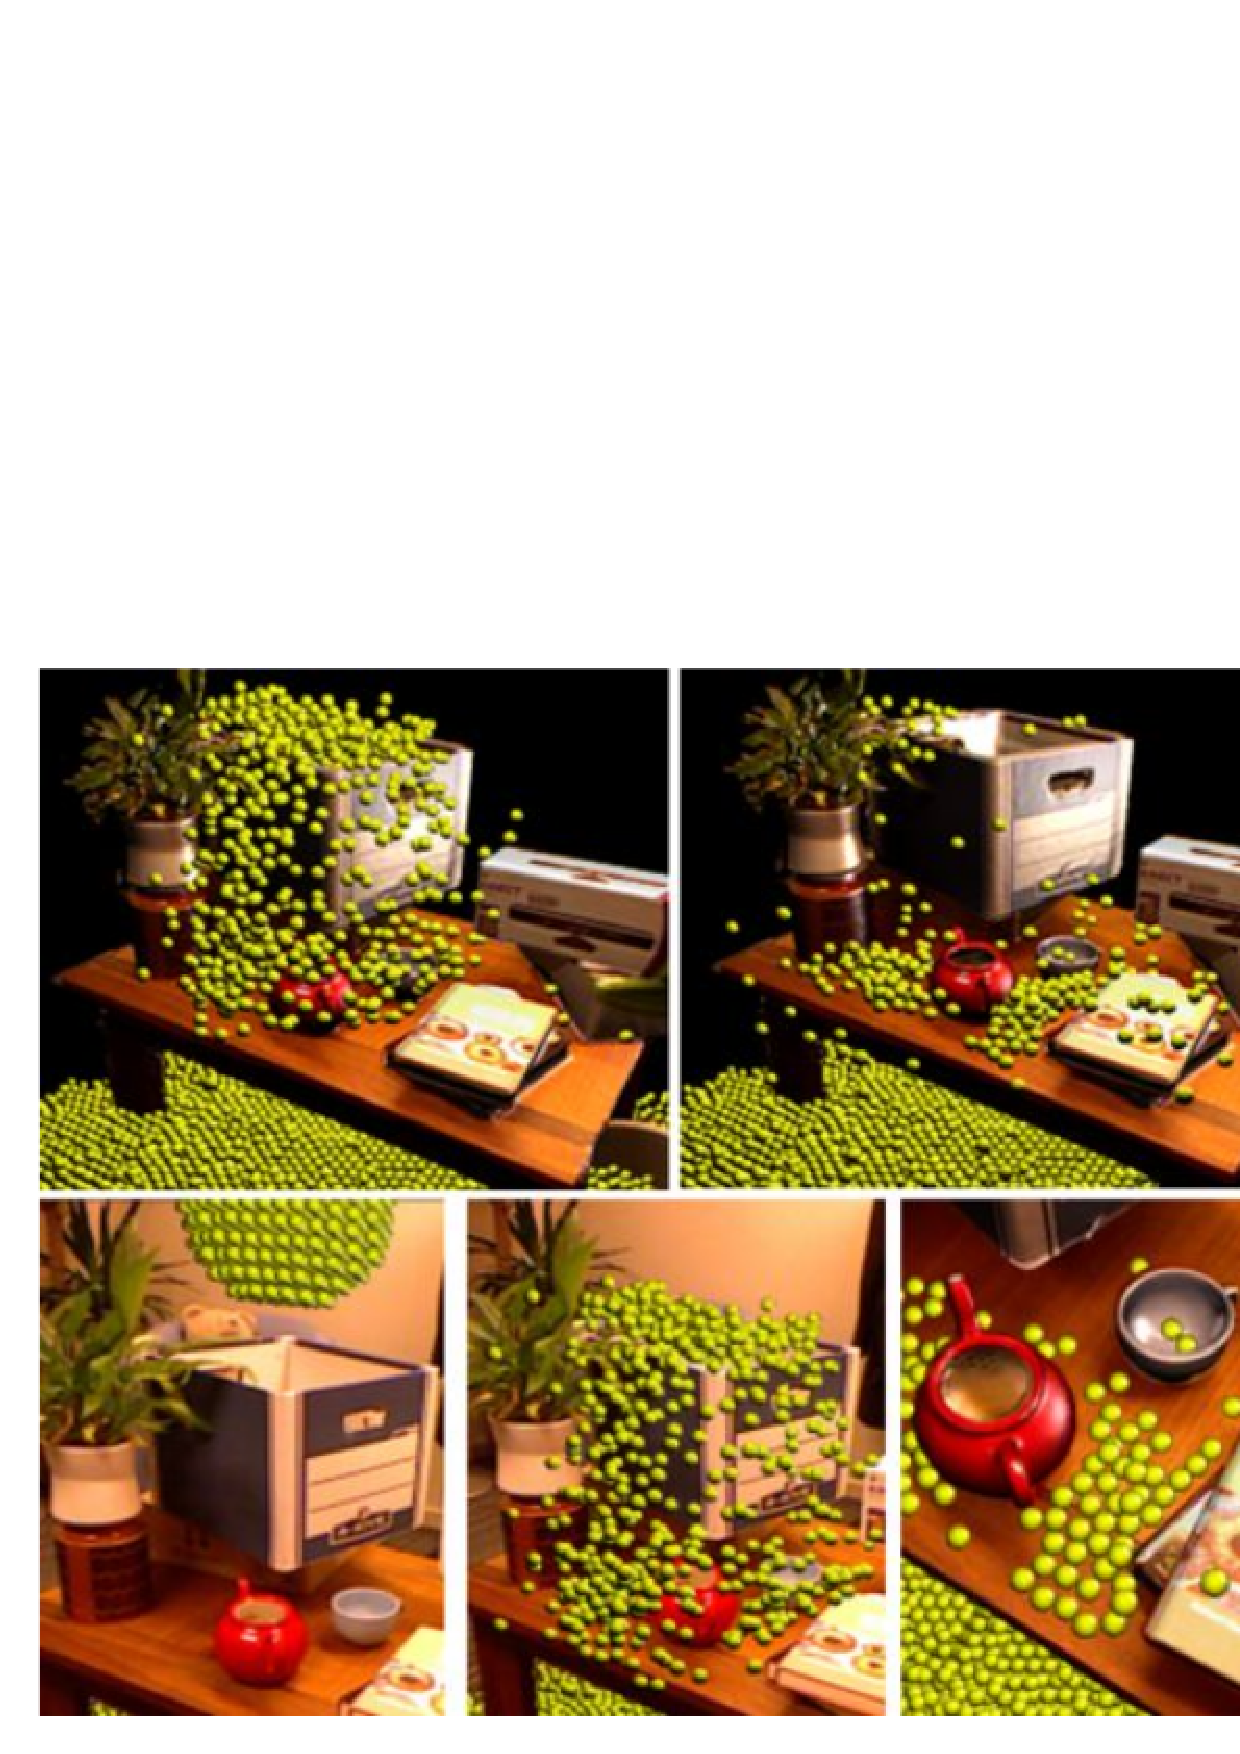
\includegraphics[scale=0.34]{images/izadi}
\caption{Reconstructed 3D scene with thousands of virtual particles}
\label{fig:izadi}
\end{center}
\end{figure}


All the 3D reconstruction methods can have problems with non lambertian 
surfaces and they need to make some assumptions about the surfaces reflectance. For example if we are using 
an infrared structured light pattern depth camera and the object that we are registering absorbs the infrared light, 
the reconstruction will fail. Similar problems can occur with laser scanners. 
Some materials such as glass or water can ruin the reconstruction.


%must be correctly located
In \cite{weise08} the user move the object using his hands in front of an RGB-D sensor (In-hand modeling), the hands are 
eliminated using a color skin detector and the user can see the reconstruction in real time, in order to correctly 
move the object.  The object is registered with Fast ICP, which instead of searching for the closest 
point, projects a transformated source point on the 2D target depth image in order to perform the matching. They use point
 to plane distance. This ICP variation is also used in \cite{jaeggli03}. \cite{weise08} uses geometrical and visual 
information to perform a correct registration. Imposing geometrical contraints based on the cameras lines of sight and visual 
contraints applying Gaussian derivative kernels to both images and measuring similarities.







\chapter{Registration}
\index{Registration}
One of the first fundamental steps to reconstruct a 3D scene is the 
positioning of the 3D points on a common coordinate system, conserving 
the original scene structure. This step is called registration. 

In general, when the sensor is collecting the 3D points from the scene, 
 its necessary to move or rotate it in order to capture new objects and surfaces from 
the scene, adding more information to the reconstructed scene. But in order to be 
able to infer the correct position of each capture, is necessary to have part 
of the view in common between two captures (an overlaping area). Thus is posible 
to position a new capture with respect to an old one in the scene, using this overlaping 
area to correctly align both captures.
 
The overlaping areas of the different captures of a scene must be correctly 
aligned when registering the points in a common coordinate system, 
thus with each new capture more information is added to the scene, 
getting closer to the desired result. 

The most used algorithm for solve this problem is called 
ICP (Iterative Closest Point) Algorithm. Given two point clouds, 
this algorithm find the best rigid transformation to align both clouds 
(minimize distance between puntos emparejados). In order to make this, 
the algorithm starts with an initial guess of the transformation. 
At each iteration the algorithm matchs points of each cloud and then 
find the best transformation. 





 


There are several techniques to track an object. If there is information about the object of interest the problem 
can be simplyfied using this information to restrict the search space, for example to certain color or shape.
 By the other hand if the object to track is unknown, it is necessary to find a more general feature, that is 
more likely to be found on the unknown interest objects. The corners are good features for this purpose. A corner 
is a point on the image where there are gradient variations on two orthogonal directions.

The most common definition of a corner is gived by Harris :

$$
E(u,v) = \begin{bmatrix} u & v \end{bmatrix} \sum\limits_{x,y} w(x,y) \begin{bmatrix} {I_x}^2 & I_x I_y \\ I_x I_y & {I_y}^2 \end{bmatrix} \begin{bmatrix} u \\ v \end{bmatrix}
$$

We loop over a neighboorhood defined by different values of (x,y) and calculate 
the difference of each pixel located at (x,y) with some other pixel located at (x+u,y+v). 
The function w(x,y) is used to give some weight to each pixel. 


Optical Flow

The optical flow methods are used to calculate motion between two sucesive image frames which are taken
 at two different times: t and \delta t.

This methods have three main supositions about the frames:

1.- The intensity remains constant
2.- They are geometricaly consistent
3.- There is a rigid transformation between one frame and the next

There are two kinds of optical flow: dense and sparse. Dense optical flow means  calculate direction vector for each pixel of the image and sparse optical flow is calculate direction vector just those pixels of the image 
who satisfy certain conditions.

Dense optical flow is computationally expensive and its difficult to find the direction vector for plain color areas. For example an image of a white paper, there are a lot of pixels with the same properties and its necesary to perform some kind of interpolation to lidiar with this pixels. By the other hand, sparse optical flow just consider pixels with more odds of been matched between the two frames.






\section{Iterative Closest Point}

The ICP (Iterative Closest Point) algorithm \cite{mckay92} is widely used for 3D Reconstruction. This algorithm tries to find 
the optimal rotation and translation between two sets of points (point clouds) that minimizes the distance between corresponding 
points. Corresponding points are determined assigning to each point of one cloud, the closest point in the other cloud.

As result at each iteration we have a set of pairs of closest points, where each pair contains one point of each cloud. This set 
of pairs changes from iteration to iteration, since the rotation and translation updates the points of one of the point clouds. If enough correct 
corresponding points are find in each iteration, the algorithm converges to the correct transformation that aligns both point clouds.


%\tiny
R : 3x3 Rotation matrix

t : 3x1 Translation vector

A,A',B : Point sets $\in R^3$

p : Pair set

%\small
\begin{algorithm}
\caption{ICP algorithm}
\begin{algorithmic}[1]
\State init(R,t)
\State A' $\leftarrow$ transform(A,R,t) 
\State p $\leftarrow$ closestPoints(A',B)
\State $\{R,t\} \gets$ updateTransformation(p)
\State $e_i = meanSquareError(p)$
\If {$e_i < umbral$ OR  $i > maxIteracions$} 
	\State return R,t
\Else
	\State go to step 2
\EndIf
\end{algorithmic}
\end{algorithm}


We want to find R and t that minimizes the following expression:

$$ \sum\limits_{i=1}^n ||R a_i -  b_i - t ||^2 $$

Where each $a_i,b_i$ is a vector $\in \mathbb{R}^3$, R is a 3x3 rotation matrix and t is a vector $\in \mathbb{R}^3$


We make a change of coordinates, placing the centroid of each cloud as origin:



\begin{align*}
 \bar{a} = \frac{1}{n} \sum\limits_{i=1}^n {a_i} \\ 
  \bar{b} = \frac{1}{n} \sum\limits_{i=1}^n {b_i} \\  
   {a'}_i = a_i - \bar{a}\\
   {b'}_i = b_i - \bar{b} 
\end{align*}

Replacing

\[ \sum\limits_{i=1}^n ||R a_i -  b_i - t ||^2 = \sum\limits_{i=1}^n ||R ( {a'}_i + \bar{a} ) -  ( {b'}_i  + \bar{b} ) - t ||^2  \]

The desired translation is $t = R \bar{a} - \bar{b} $. We must consider the rotation in this expression, since 
the rotation of a cloud will change the position of all points and as consecuence the translation.

Replacing t in our previous expression we get:
\begin{flalign*}
&\sum\limits_{i=1}^n ||R a'_i - b'_i ||^2  \\ 
&=\sum\limits_{i=1}^n (R a'_i - b'_i)^t (R a'_i - b'_i) \\
&=\sum\limits_{i=1}^n ( (R a'_i)^t R a'_i - (R a'_i)^t b'_i  - b_i^{\prime t} R a'_i + b_i^{\prime t} b'_i) \\
&=\sum\limits_{i=1}^n ( a_i^{\prime t} R^t R a'_i - 2 b_i^{\prime t} R a'_i + b_i^{\prime t} b'_i) \\ 
&=\sum\limits_{i=1}^n (a_i^{\prime t} a'_i -  2 b_i^{\prime t} R a'_i + b_i^{\prime t} b'_i) 
\end{flalign*}


Minimize the previous expression is equivalent to maximize:

\begin{align*}
& \sum\limits_{i=1}^n b_i^{\prime t} R a'_i =  Trace ( \sum\limits_{i=1}^n R a'_i  b_i^{\prime t} ) = Trace (RH) \\
& H=\sum\limits_{i=1}^n a'_i  b_i^{\prime t} 
\end{align*}


\begin{mybox}{gray}{Lemma}
For any positive definite matrix $A A^t$ and any orthogonal matrix B 

\[ Trace( A A^t ) \geq Trace (B A A^t) \]

\end{mybox}


Proof of lemma:

Let $a_i$ be the ith column of A, then:

\begin{align*}
Trace( B A A^t ) = Trace (A^t B A) = \sum\limits_i a_i^t B a_i 
\end{align*}

But by the Schwarz inequality

\[ a_i^t B a_i \leq \sqrt{ a_i^t a_i (a^t B^t B a_i)} = a^t a_i \]


Now using this lema we will maximize our expression:


Lets apply the SVD factorization to H, then:

\[ H = U \Sigma V^t \]

Where U and V are 3x3 orthonormal matrices and $\Sigma$ is a diagonal matrix with no negative elements.

Let $ R = V U^t $ then :

\begin{align*}
RH = VU^t U \Sigma V^t = V \Sigma V^t = V \Sigma^{\frac{1}{2}} (V \Sigma^{\frac{1}{2}})^t
\end{align*}

Which is symetrical and positive definite.
Therefore from Lemma, for any 3x3 orthonormal matrix B

\[ Trace( R H ) \geq Trace( B R H ) \]

Thus the solution for our problem is 

\begin{align*}
R = V U^t \\
t = R \bar{a} - \bar{b}
\end{align*}


This means that if we apply the rotation R and the translation t, to each point of the point cloud A, the distance between closest points of 
transformed point cloud A with point cloud B will be minimal. When registering a set of points from a real 3D scene it allows to obtain a correct 
align between sucesive scene captures.

\section{Proposed Algorithm}

\subsection{Proposed ICP Algorithm}

\begin{algorithm}
\caption{Proposed ICP algorithm}
\begin{algorithmic}[1]
\State estimate $R_1,t_1$ using SURF
\State estimate $R_2,t_2$ using Optical Flow
\State calculate $P_1$ applying photoconsistency method with $R_1,t_1$
\State calculate $P_2$ applying photoconsistency method with $R_2,t_2$
\State set $R,t$ as $R_1,t_1$ if $P_1$ is minor than $P_2$, set as $R_2,t_2$ in other case.
\State A = edgeFilter(A)
\State B = edgeFilter(B)
\State A' $\leftarrow$ transform(A,R,t) 
\State p $\leftarrow$ closestPoints(A',B)
\State $\{R,t\} \gets$ updateTransformation(p)
\State $e_i = meanSquareError(p)$
\If {$e_i < umbral$ OR  $i > maxIterations$} 
	\State return R,t
\Else
	\State goto step 8
\EndIf
\end{algorithmic}
\end{algorithm}


In the first step the proposed algorithm uses SURF and optical flow to obtain two candidate estimations of 
R,t for the first iteration of the ICP algorithm. For each pair of consecutive RGB images optical flow 
 and SURF are applied, obtaining pairs of correspondences between both captures. 

SURF and optical flow work on the 2D image space, but using 
the 3D information from the depth map its possible to get the 3D position 
of the each pair of correspondences respect to the camera. 

Having pairs of 3D points, one point of the capture at time t and other point 
of the capture at time t + 1 its possible to obtain the rotation R and translation t
 that minimizes the distances between the correspondences. Obtaining an initial guess 
 for ICP. Then both estimations (optical flow and SURF) are compared using the photoconsistency measure, choosing 
the estimation with less photometric error.

A photoconsistency measure is used to compare the quality of the initial estimations of the sensor
 position and orientation. A good estimation of the relative transform between two captures, implies 
a small diference between the first RGB image projected using the relative transform and the second RGB 
image. Using this calculation we can detect if ICP guess is good or not.


\subsection{Complete process}

\begin{figure}[!h]
\begin{center}
\includegraphics[scale=0.55]{images/graph_icp}
\caption{All constraints are generated using the proposed ICP.}
\end{center}
\end{figure}


The complete registration process can be described by the following algorithm:

\begin{algorithm}
\caption{General algorithm}
\begin{algorithmic}[1]
\State read prevFrame
\State globalTransf=4x4MatrixIdentity()
\State addGraphVertex(globalTransf)
\While {read frame} 
\State globalTransf=proposedICP(frame,prevFrame)*globalTransf
\State addGraphVertex(globalTransf)
\State addGraphEdge(frame,prevFrame)
\ForAll {oldFrame previous to prevFrame } 
\State detectLoop(frame,oldFrame)
\If {loopDetected}
\State addGraphEdge(frame,oldFrame)
\EndIf
\EndFor
\EndWhile
\end{algorithmic}
\end{algorithm}

Consecutive frames are readed and then both point clouds are filtered, removing plain surfaces, thus obtaining point clouds 
with a lesser amount of points. With this ICP will work on point clouds that contains around 
only 10\% or 20\% of the original points depending on the scene. But this points are highly representative for registration purposes.

Finally, the classical ICP algorithm is applied to the point clouds.

A graph is generated in the process. Adding spatial restrictions between sucesive frames and also between non-sucesive but similar 
frames. In order to reduce drift with a graph optimization approach.

\begin{algorithm}
\caption{AddGraphEdge algorithm}
\begin{algorithmic}[1]
\State [R,t] = proposedICP(framei,framej)
\State photoCons = photoConsistency(framei,framej,R,t)
\State informationMatrix=Identity6x6*photoCons;
\State graph.addEdge(i,j,R,t,informationMatrix)
\end{algorithmic}
\end{algorithm}

Note: the graph optimization algorithm internally works with quaternions instead of rotation matrices.



 







\chapter{Results and Discussion}
%\chapter{Point Features}
%\index{Point Features}
%
A point feature is some characteristic that identifies the point and is desirable 
that points with geometrical similarities share similar features. For example..

\section{Point Neighboorhood}

In order to talk about point features is necessary to define a neighboorhood. 

We will define a neighboordhood of a point as a set of points that are related 
with it, sharing some common properties.

k neightboorhood : the k closests points 

radious neightboorhood : all the points that are within some radious

\section{Point Normal}

A very important geometrical property of a point is the normal. 
Because it indicates the orientation of the surface that contains it,
this property is heavily used in computer graphics to compute the 
lighting of an scene, since with the normals we can simulate the 
trajectory of an light ray that is intersecting the surface.
This property is also used as a point feature.



\section{Point Curvature}

The curvature is related with normal changes in a surface, 
a surface with no curvature will have all the normals pointing 
to the same direction. 




%\chapter{RGB Tracking}
%\index{RGB Tracking}

\chapter{Conclusions}
\label{conclusions}
\index{Conclusions}
Proposed algorithm exihibit a very good performance in small trajetories (maximum 20 captures), 
most of the error is due to accumulated error. A more complete pose graph optimization algorithm 
should resolve this problem.

Using edges instead of the complete point cloud in order to perform the alineation of captures 
reduces algorithm complexity and exhibit noticeable improvements in the result. 




\appendix

\addcontentsline{toc}{chapter}{Appendix}


\chapter{Acronyms}
\label{acronyms}
\index{acronyms}
\begin{description}
\item ATE: Absolute Trajectory Error
\item EMM: Environment Measurement Model
\item ICP: Iterative Closest Point 
\item NDT: Normal Distributions Transform
\item RANSAC: Random Sample Consensus
\item RMSE: Root Mean Squared Error
\item RPE: Relative Pose Error
\item SIFT: Scale Invariant Feature Transform
\item SLAM: Simultaneous Localization and Mapping
\item SURF: Speeded Up Robust Features
\item ToF: Time of Flight
\end{description}
\vspace{\fill}\LaTeXe





\backmatter

\addcontentsline{toc}{chapter}{\bibname}
\bibliographystyle{plain}
\bibliography{tesis}

\end{document}

